% no answer key
% \documentclass[letterpaper]{exam}

% answer key
\documentclass[letterpaper, landscape]{exam}
\usepackage{2in1, lscape} 
\printanswers

% for the cent symbol
\usepackage{textcomp}

% the textcent command eats the space following the symbol
\usepackage{xspace}
\newcommand{\cent}{\textcent\xspace}

\usepackage{units} 
\usepackage{xfrac} 
\usepackage[fleqn]{amsmath}
\usepackage{cancel}
\usepackage{float}
\usepackage{mdwlist}
\usepackage{booktabs}
\usepackage{cancel}
\usepackage{polynom}
\usepackage{caption}
\usepackage{fullpage}
\usepackage{comment}
\usepackage{enumerate}
\usepackage{graphicx}
\usepackage{parskip}

\everymath{\displaystyle}


\title{Statistics \\ Homework Twelve}
\date{\today}
\author{}

\begin{document}

  \maketitle

  \section{Homework}
  \ifprintanswers
  \else
    \begin{itemize*}
      \item read Chapter 13 
      \item take a look at the ``Check Your Skills'' exercises
      \item exercises: TO DO
    \end{itemize*}
  \fi

  \ifprintanswers
    \begin{description}

      \item[22] 
        \begin{enumerate}[(a)]
          \item \fbox{ not binomial }
            The number of defects might be a normal distribution, but there
            isn't a probability of ``success'' or ``failure''

          \item \fbox{ binomial }

          \item \fbox{ binomial }
        \end{enumerate}

      \item[23]
        \begin{enumerate}[(a)]
          \item This one isn't appropriate because the sample size is small and
            the probability of success varies widely from attempt to attempt.

          \item This one is appropriate for the binomial distribution.
        \end{enumerate}

      \item[24]
        \begin{enumerate}[(a)]
          \item $n = 20$; $p = 0.25$
          \item 5
          \item $ \binom{20}{5} 0.25^5 \cdot 0.75^5 \approx \boxed{ 0.2023 } $
        \end{enumerate}

      \item[25]
        \begin{enumerate}[(a)]
          \item $n = 5$; $p = 0.5$

          \item 0 to 5

          \item see Figure \ref{fig:ex25}

            \begin{figure}[H]
              \centering
              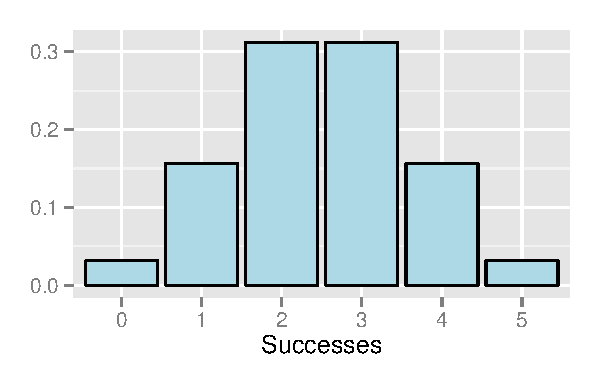
\includegraphics{ex25.pdf}
              \caption{Exercise 25}
              \label{fig:ex25}
            \end{figure}

          \item 
            \begin{align*}
              \mu    & = \boxed{ 2.5 } \\
              \sigma & = \sqrt{2.5 \cdot 0.5 \cdot 0.5} \approx \boxed{ 0.7906 } \\
            \end{align*}
        \end{enumerate}

      \item[26]
        \begin{enumerate}[(a)]
          \item 
            \begin{align*}
              \mu    & = \boxed{ 6 } \\
              \sigma & = \sqrt{6 \cdot 0.5 \cdot 0.5} \approx \boxed{ 1.2248 } \\
            \end{align*}

          \item The probability of exactly 8 is:
            \[
              \binom{12}{8} 0.5^8 \cdot 0.5^4 \approx \boxed{ 0.1208 } 
            \]

            According to my computer, the probability of at least 8 is
            approximately \fbox{ 0.1938 }

        \end{enumerate}

      % \item[27]
      %   \begin{enumerate}[(a)]
      %     \item There is a probability of success and a fixed sample size.

      %     \item 
      %       The probability of nobody getting pregnant under ideal
      %       conditions is:
      %       \[
      %         0.99^{20} \approx \boxed{ 0.8179 } 
      %       \]

      %       The probability of nobody getting pregnant under ideal
      %       conditions is:
      %       \[
      %         0.95^{20} \approx \boxed{ 0.3585 }
      %       \]
      %   \end{enumerate}

      \item[28]
        \begin{align*}
          \mu    & = 250 \\
          \sigma & = \sqrt{250 (0.5)} \\
                 & \approx 11.18 \\
        \end{align*}

        Convert 235 to a z-score:
        \[
          z_{235} = \frac{235 - 250}{11.18} \approx -1.3416
        \]

        Use table A:
        \[
          P(X \geq 235) \approx 1 - 0.0899 = \boxed{ 0.9101 }
        \]

        According to my computer, the exact binomial probability is
        approximately 0.9172

      \item[31]
        \begin{enumerate}[(a)]
          \item 
            \[
              \binom{8}{6} 0.75^6 \cdot 0.25^2 \approx \boxed{ 0.3115 } 
            \]

          \item \fbox{ $\mu = 0.75 \cdot 80 = 60$ }

          \item Since 60 is the mean, there is a \fbox{ 0.5 } probability of a
            result of at least 60 using the Normal distribution.

            According to my computer, the exact binomial probability is
            approximately 0.5597

        \end{enumerate}

      \item[32]
        \begin{enumerate}[(a)]
          \item This is a binomial distribution with 
            \fbox{ $n = 1000$ and $p = 0.004$ }

          \item $\mu = 1000 \cdot 0.004 = \boxed{ 4 }$

          \item $np = 4 < 10$. The Normal approximation should only be used when
            $np \geq 10$.
        \end{enumerate}

      \item[34]
        \begin{enumerate}[(a)]
          \item
            \begin{align*}
              \mu    & = 0.13 \cdot 1200 = \boxed{ 156 } \\
              \sigma & = \sqrt{156 \cdot 0.13 \cdot 0.87} \approx \boxed{ 4.2 } \\
            \end{align*}

          \item 95\% of the time the sample will be with 2 standard deviations
            of the mean. So 95\% of the time, the result will contain somewhere
            \fbox{ between 148 and 164 } Hispanics.

          \item 
            \begin{align*}
              0.13 n & = 200 \\
              n      & \approx \boxed{ 1539 } \\
            \end{align*}
        
        \end{enumerate}

      \item[35]
        \begin{enumerate}[(a)]
          \item
            With 100 questions:

            \begin{align*}
              \mu    & = 0.75 \cdot 100 = 75 \\
              \sigma & = \sqrt{75 \cdot 0.75 \cdot 0.25} \approx 3.75 \\
            \end{align*}

            convert to z-scores:
            \begin{align*}
              z_{70} &= \frac{70 - 75}{3.75} \approx -1.33 \\
              z_{80} &= \frac{80 - 75}{3.75} \approx 1.33 \\
            \end{align*}

            From Table A:
            \begin{align*}
              P(X < 70) & \approx 0.0912 \\
              P(X < 80) & \approx 0.9087 \\
              \\
              P(70 < X < 80) & \approx 0.9087 - 0.0912 \\
                             & = 0.8176 \\
            \end{align*}

          \item
            With 200 questions:

            \begin{align*}
              \mu    & = 0.75 \cdot 200 = 150 \\
              \sigma & = \sqrt{150 \cdot 0.75 \cdot 0.25} \approx 5.303 \\
            \end{align*}

            convert to z-scores:
            \begin{align*}
              z_{70\%} &= \frac{140 - 150}{5.303} \approx -1.886 \\
              z_{80\%} &= \frac{160 - 150}{5.303} \approx 1.866 \\
            \end{align*}

            From Table A:
            \begin{align*}
              P(X < 140) & \approx 0.0296 \\
              P(X < 160) & \approx 0.9704 \\
              \\
              P(140 < X < 160) & \approx 0.9704 - 0.0296 \\
                               & = 0.9407 \\
            \end{align*}
        
          \item[36]
            \begin{align*}
              \mu    & = 0.5 \cdot 10,000 = 5000 \\
              \sigma & = \sqrt{5000 \cdot 0.5 \cdot 0.5} \approx 35.36 \\
            \end{align*}

            convert the actual result to a z-score:
            \begin{align*}
              z_{max} &= \frac{5067 - 5000}{35.56} \approx 1.895 \\
              z_{min} &= \frac{4933 - 5000}{35.56} \approx -1.895 \\
            \end{align*}

            From Table A:
            \begin{align*}
              P(X > 5067) & \approx 0.2965 \\
              P(X < 4933) & \approx 0.0290 \\
              P(X < 4933 \text{ or } X > 5067 &\approx \boxed{ 0.06 } \\
            \end{align*}

            The coin may have been slightly biased towards heads.

        \item[38]
          You can't use the Normal approximation for this problem because the
          sample size is too small.

          \begin{enumerate}[(a)]
            \item 
              $\mu = 0.05 \cdot 20 = \boxed{ 1 }$

              \begin{align*}
                P(X = 0) & = 0.95^{20} \\
                         & \approx 0.3585 \\
                P(X = 1) & = \binom{20}{1} 0.05 \cdot 0.95^{19} \\
                         & \approx 0.3774 \\
                P(X = 2) & = \binom{20}{2} 0.05^2 \cdot 0.95^{18} \\
                         & \approx 0.1887 \\
                         \\
                P(X \leq 2) & \approx 0.3585 + 0.3774 + 0.1887 \\
                            & = \boxed{ 0.9245 }
              \end{align*}

            \item 
              $\mu = 0.95 \cdot 20 = \boxed{ 19 }$

              \begin{align*}
                P(X = 20) & = 0.95^{20} \\
                          & \approx 0.3585 \\
                P(X = 19) & = \binom{20}{1} 0.05 \cdot 0.95^{19} \\
                          & \approx 0.3774 \\
                P(X = 18) & = \binom{20}{2} 0.05^2 \cdot 0.95^{18} \\
                          & \approx 0.1887 \\
                         \\
                P(X \geq 18) & \approx 0.3585 + 0.3774 + 0.1887 \\
                             & = \boxed{ 0.9245 }
              \end{align*}

          \end{enumerate}

        \item[39]
          \begin{enumerate}[(a)]
            \begin{align*}
              \mu &= 0.95 \cdot 1400 = 1330 \\
              \sigma &= \sqrt{1330 \cdot 0.95 \cdot 0.05} \approx 7.95 \\
            \end{align*}

            75\% of the students is only 1050 students. Convert to z-score:
            \[
              z = \frac{1050 - 1330}{7.95} \approx -35
            \]

            There is essentially zero chance of less than 75\% of the students
            contracting the disease.

          \end{enumerate}

      \end{enumerate}
  \end{description}

  \else
    \vspace{11 cm}
    \begin{quote}
      \begin{em}
        TO DO
      \end{em}
    \end{quote}
    \hspace{1 cm}--Marcus Aurelius
  \fi

\end{document}

